\documentclass[usenames,dvipsnames,notes,11pt,aspectratio=169,hyperref={colorlinks=true, linkcolor=blue}]{beamer}
\usepackage{ifthen}
\usepackage{xcolor}
\usepackage{pgfplots}
\usepackage{amsmath}
\usepackage{centernot}
\usepackage{pifont}
\usepackage{tabularx}
\usepackage{makecell}
\usepackage{cuted}
\usepackage{booktabs}
\usepackage{array}
\usepackage{textcomp}
\usepackage{setspace}
\usepackage{xspace}
\usepackage{subcaption}
\usepackage{tikz}
\usepackage{pdfcomment}
%\newcommand{\pdfnote}[1]{\marginnote{\pdfcomment[icon=note]{#1}}}
\newcommand{\pdfnote}[1]{}

\usepackage{pgfpages}
%\setbeameroption{show notes on second screen}


\input ../beamer-style
\input ../std-macros
\input ../macros

\newcommand{\pt}{\partial}

\AtBeginSection[]
{
    \begin{frame}
        \frametitle{Table of Contents}
        \tableofcontents[currentsection]
    \end{frame}
}
\parskip=10pt

\title[CSCI-GA.2590]{Neural Sequence Generation}
\author[He He]{He He
}
\institute[NYU]{
    
\includegraphics[height=1cm]{../figures/nyu-logo}\\
}
\date{February 14, 2023}

\begin{document}
\begin{frame}
\titlepage
\end{frame}

\begin{frame}
    {Sequence generation}
    \begin{itemize}[<+->]
        \item Text classification: $h: \sV^n \rightarrow \pc{0,\ldots,K}$
        \item Sequence generation: $h: \sV_{\text{in}}^n \rightarrow \sV_{\text{out}}^m$
            \begin{itemize}[<.->]
                \item Summarization: document to summary
                \item Open-domain dialogue: context to response
                \item Parsing: sentence to linearized trees
                \item In general: text to text
            \end{itemize}
    \end{itemize}
   
    \pause{
        Main difference (and challenge) is that the output space is much larger.}
\end{frame}

\begin{frame}
    {Reduce generation to classification}
    Setup:\\
    \begin{itemize}
        \item Input: $x \in \sV_{\text{in}}^n$, e.g. \textit{Le Programme    a    ate    mis    en application}
        \item Output: $y \in \sV_{\text{out}}^m$, e.g., \textit{The program has been implemented }
    \end{itemize}
    \pause

    Consider a probabilistic model $p(y\mid x)$\\
    \begin{itemize}[<+->]
        \item Can we reduce it to classification (think logistic regression)?
        \item Decompose the problem using \textbf{chain rule of probability} 
            \begin{align*}
                p(y\mid x) &= p(y_1\mid x)p(y_2\mid y_1, x)\ldots p(y_m\mid y_{m-1},\ldots,y_1, x) \\
                &= \prod_{i=1}^m p(y_i\mid y_{<i}, x)
            \end{align*}
        \item We only need to model the \blue{next word distribution} $p(y_i\mid y_{<i}, x)$ now.
    \end{itemize}
\end{frame}

\begin{frame}
    {Reduce generation to classification}
    We want to model the {next word distribution} $p(\red{y_i}\mid \blue{y_{<i}}, \green{x})$.\\
    \begin{itemize}[<+->]
        \item Input: a sequence of tokens (\blue{prefix} and \green{input})
        \item Output: the \red{next word} from the output vocabulary
        \item We have reduced it to a classification problem.
    \end{itemize}

    \pause
    We can use an RNN to model $p(y_i\mid {y_{<i}}, {x})$.
    \begin{figure}
        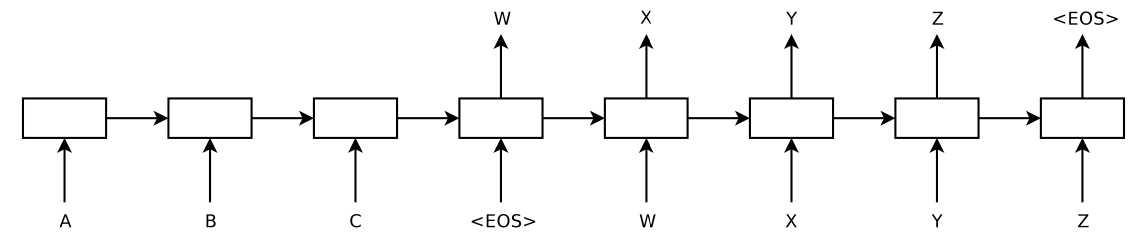
\includegraphics[height=2.5cm]{figures/s2s-ilya}
        \caption{From \href{https://arxiv.org/abs/1409.3215}{Sequence to Sequence Learning with Neural Networks} [Sutskever et al., 2014]}
    \end{figure}
\end{frame}

\begin{frame}
    {The encoder-decoder architecture}
    \begin{figure}
        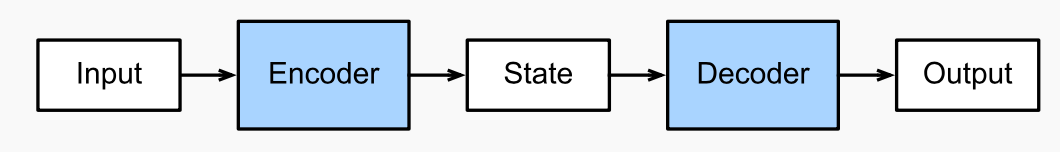
\includegraphics[height=1.5cm]{figures/enc-dec}
        \caption{10.6.1 from \href{https://d2l.ai/chapter_recurrent-modern/encoder-decoder.html}{d2l.ai}}
    \end{figure}
    \vspace{-1em}

    Model the {input} (e.g., French) and the {output} (e.g., English) separately.\\
    \pause
    \begin{itemize}
        \item The \textbf{encoder} reads the input:
            $$
            \mathrm{Encoder}(x_1,\ldots,x_n) = \pb{h_1,\ldots,h_n}$$ where $h_i\in\BR^d$
        \item The \textbf{decoder}  writes the output:
            $$\mathrm{Decoder}(h_1,\ldots,h_n) = \pb{y_1,\ldots, y_m}$$.
    \end{itemize}
\end{frame}

\begin{frame}
    {RNN encoder-decoder model}
    \begin{figure}
        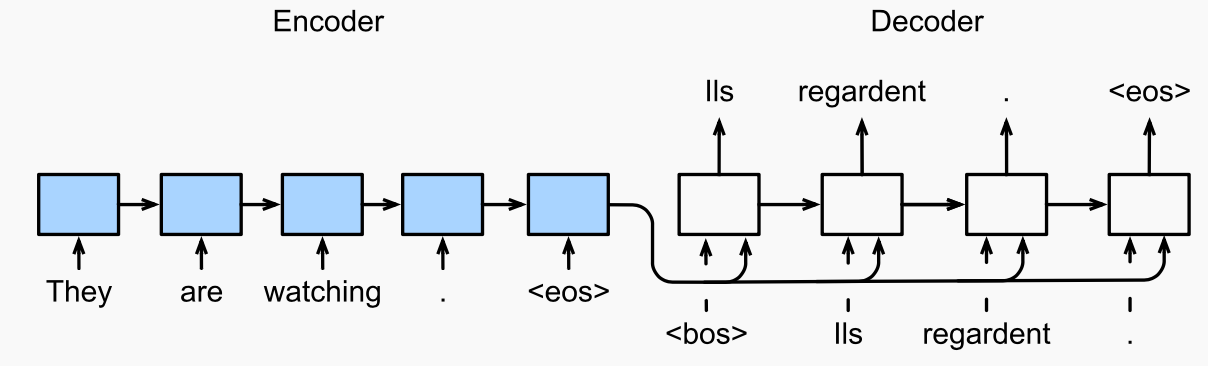
\includegraphics[height=2.5cm]{figures/rnn-enc-dec}
        \caption{10.7.1 from \href{https://d2l.ai/chapter_recurrent-modern/seq2seq.html}{d2l.ai}}
    \end{figure}
    \vspace{-1em}

    \begin{itemize}
        \item The \textbf{encoder} embeds the input recurrently
            and produce a \textbf{context vector}
            $$
            h_t = \mathrm{RNNEncoder}(x_t, h_{t-1}), \quad
            c = f(h_1,\ldots,h_n)
            $$
        \item The \textbf{decoder}  produce the output state {recurrently}
            and map it to a distribution over tokens
            $$s_t = \mathrm{RNNDecoder}(\pb{y_{t-1};c}, s_{t-1}), \quad
            p(y_t\mid y_{<t}, c) = \mathrm{softmax}(\mathrm{Linear}(s_t))
            $$
    \end{itemize}
\end{frame}

\begin{frame}
    {Bi-directional RNN encoder}
    The $\text{[Forbes]}_{??}$ building is at 60 Fifth Ave.
    \pause

    Each hidden state should summarize both \blue{left and right context}
    \pause

    \medskip
    \begin{columns}
        \begin{column}{0.5\textwidth}
    \begin{figure}
        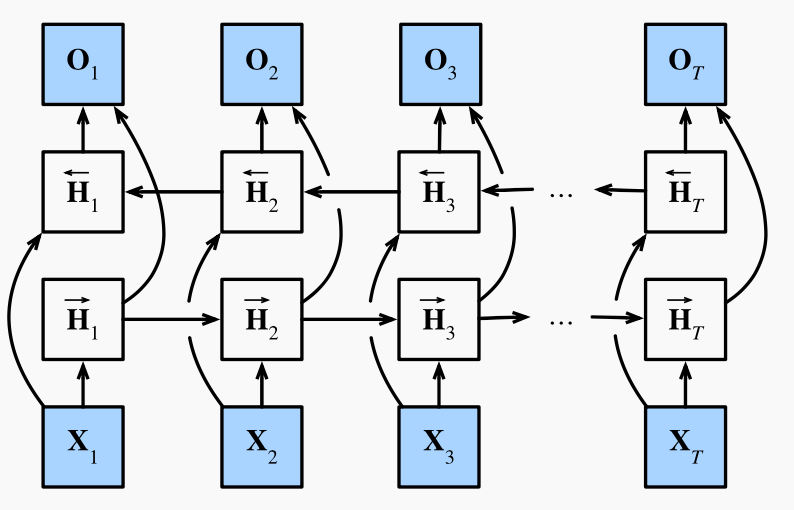
\includegraphics[height=3.5cm]{figures/birnn}
        \caption{10.4.1 from \href{https://d2l.ai/chapter_recurrent-modern/bi-rnn.html}{d2l.ai}}
    \end{figure}
        \end{column}
        \begin{column}{0.5\textwidth}
            \begin{itemize}
                \item Use two RNNs, one encode from left to right, the other from right to left
                \item Concatenate hidden states from the two RNNs
            \begin{align*}
                h_t &= [\overleftarrow{h_t}; \overrightarrow{h_t}]\\
                o_t &= Wh_t + b
            \end{align*}
            \end{itemize}
        \end{column}
    \end{columns}
\end{frame}

\begin{frame}
    {Multilayer RNN}
    \begin{columns}
        \begin{column}{0.5\textwidth}
    \begin{figure}
        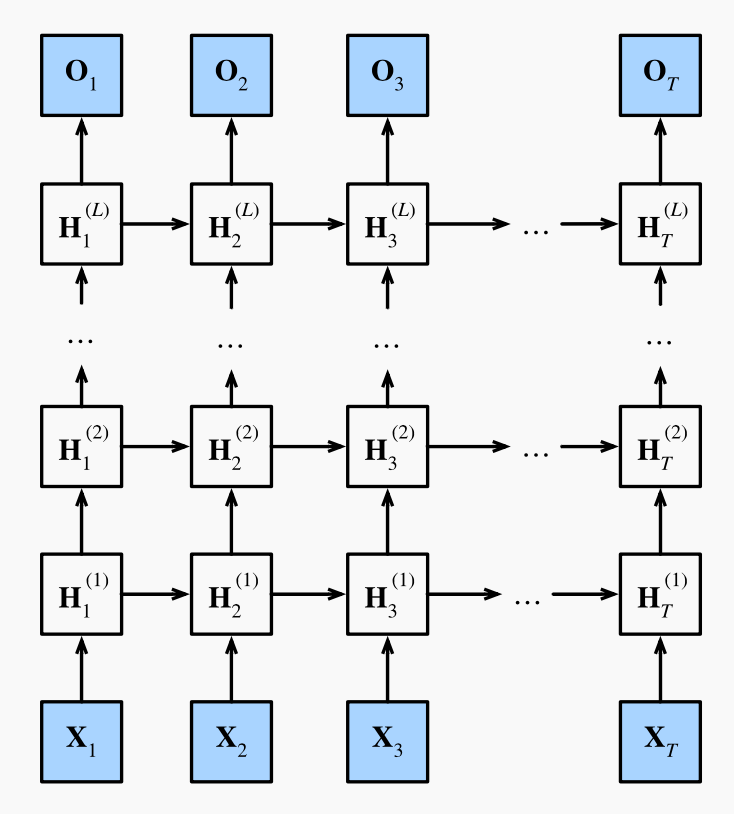
\includegraphics[height=4.5cm]{figures/multi-rnn}
        \caption{\href{https://d2l.ai/chapter_recurrent-modern/deep-rnn.html}{10.3.1} from {d2l.ai}}
    \end{figure}
        \end{column}
        \begin{column}{0.5\textwidth}
            \begin{itemize}
                \item Improve model capacity (scaling up) 
                \item Inputs to layer 1 are words
                \item Inputs to layer $l$ are outputs from layer $l-1$
                \item Typically 2--4 layers
            \end{itemize}
        \end{column}
    \end{columns}
\end{frame}

\begin{frame}
    {Encoder-decoder attention}
    \textbf{Motivation}: should we use the same context vector for each decoding step?

    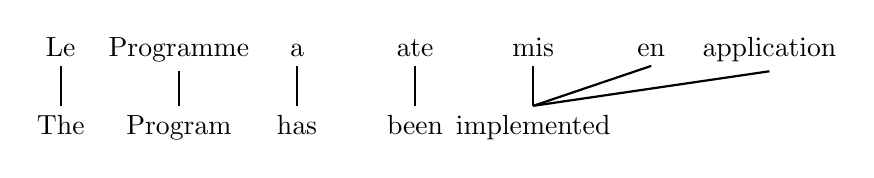
\begin{tikzpicture}
        \foreach \i/\w in {1/Le, 2/Programme, 3/a, 4/ate, 5/mis, 6/en, 7/application}{
            \node[anchor=base] (x\i) at(1.5*\i,0) {\w};
        }
        \foreach \i/\w in {1/The, 2/Program, 3/has, 4/been, 5/implemented}{
            \node[anchor=base] (y\i) at(1.5*\i,-1) {\w};
        }
        \path[draw, thick] (x1.south) -- (y1.north);
        \path[draw, thick] (x2.south) -- (y2.north);
        \path[draw, thick] (x3.south) -- (y3.north);
        \path[draw, thick] (x4.south) -- (y4.north);
        \path[draw, thick] (x5.south) -- (y5.north);
        \path[draw, thick] (x6.south) -- (y5.north);
        \path[draw, thick] (x7.south) -- (y5.north);
    \end{tikzpicture}

    We may want to ``look at'' different parts of the input during decoding.

    \pause
    \begin{columns}
        \begin{column}{0.6\textwidth}
    Think the database analogy:\\
    \begin{itemize}[<+->]
        \item Query: decoder states $s_{t-1}$
        \item Key: encoder states $h_1,\ldots,h_n$
        \item Value: encoder states $h_1,\ldots,h_n$
        \item Attention context: $c_t = \sum_{i=1}^n \alpha(s_{t-1}, h_i) h_i$
        \item Next state: $s_t = \mathrm{RNNDecoder}(\pb{y_{t-1};c_t}, s_{t-1})$
    \end{itemize}
        \end{column}
        \begin{column}{0.4\textwidth}
            \onslide<+->{
            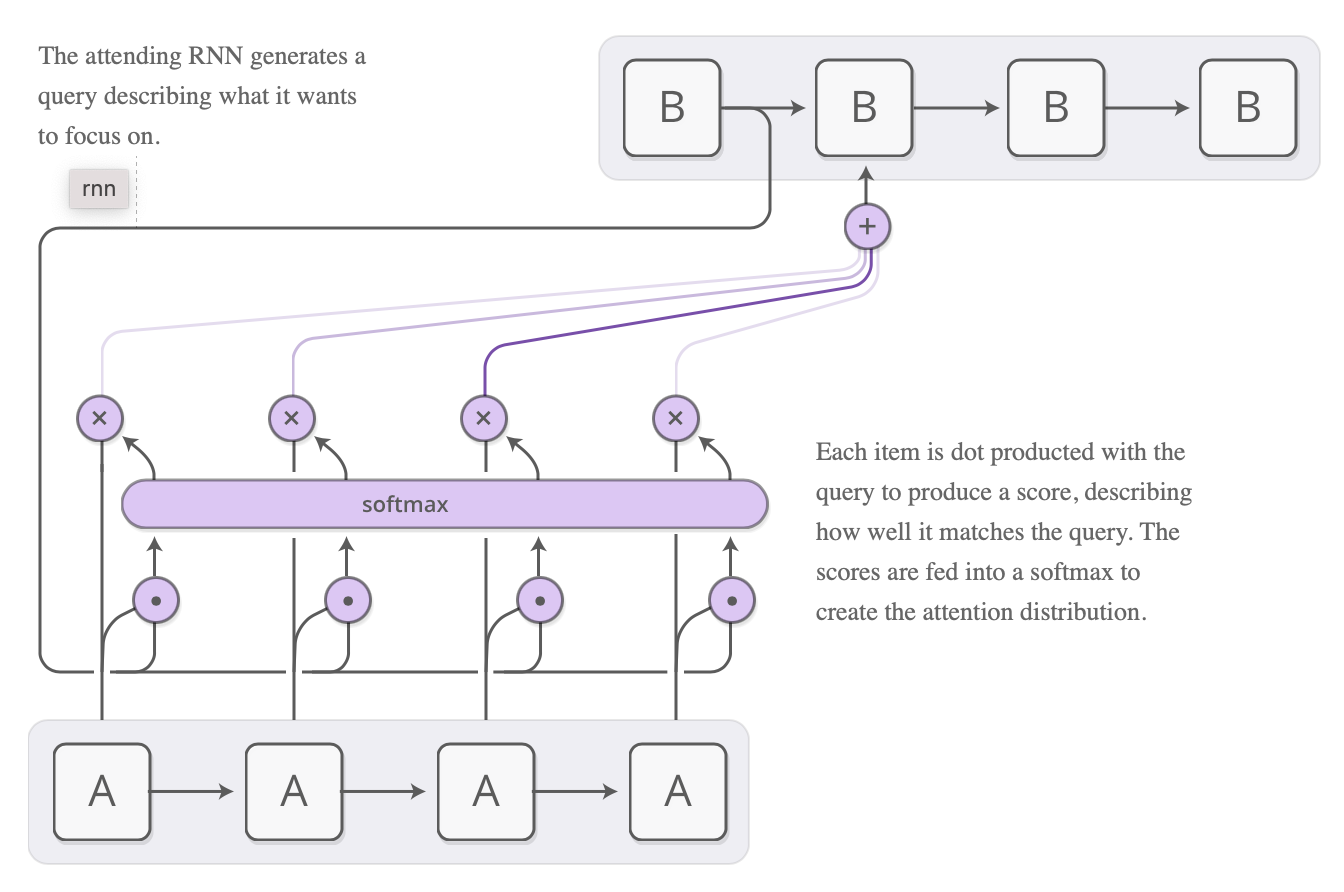
\includegraphics[height=4cm]{figures/s2s-attention}
            }
        \end{column}
    \end{columns}
\end{frame}

\begin{frame}
    {Summary so far}
    The outputs of an encoder can be used by linear classifiers for classification, sequence labeling etc.

    A decoder is used to \blue{generate} a sequence of symbols.

    RNN encoder decoder model:\\
    \begin{itemize}
        \item Basic unit is an \blue{RNN} (or its variants like LSTM)
        \item Make it more expressive: \blue{bi-directional}, \blue{multilayer} RNN
        \item \blue{Encoder-decoder attention} helps the model learn input-output dependencies more easily
        \item Bi-directional LSTM is the go-to architecture for NLP tasks until around 2017
    \end{itemize}
\end{frame}

\begin{frame}
    {Transformer encoder decoder model}
    \begin{figure}
        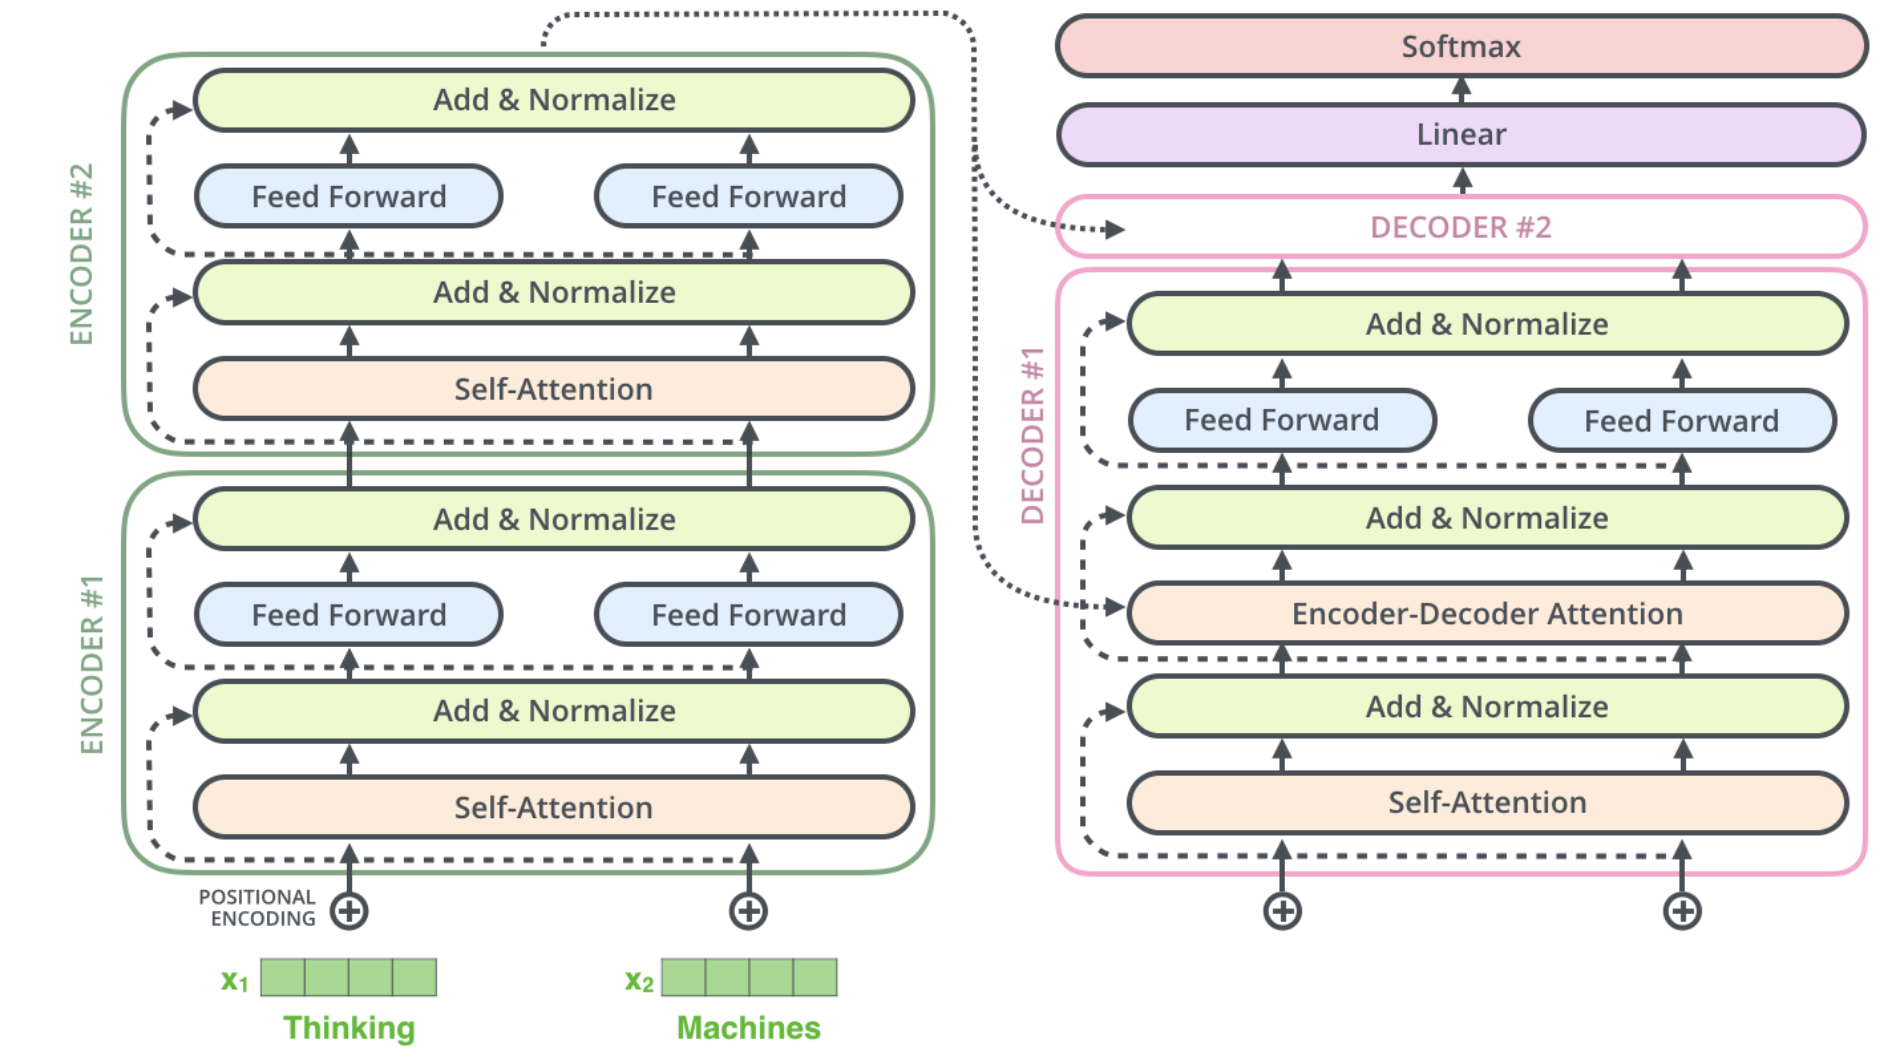
\includegraphics[height=5cm]{figures/transformer-enc-dec}
        \caption{From \href{https://jalammar.github.io/illustrated-transformer/}{illustrated transformer}}
    \end{figure}
    \vspace{-2em}

    \begin{itemize}
        \item Stack the tranformer block (typically 12--24 layers)
        \item Decoder has an additional encoder-decoder multi-head attention layer
    \end{itemize}
    \pause\vspace{-1ex}
    %\think{Which part of the computation can be parallelized?}
\end{frame}

\begin{frame}
    {Impact on NLP}
    \begin{itemize}
        \item Initially designed for sequential data and obtained SOTA results on MT
        \item Replaced recurrent models (e.g. LSTM) on many tasks
        \item Enabled large-scale training which led to pre-trained models such as BERT and GPT-2 (in two weeks)
    \end{itemize}
\end{frame}


\begin{frame}
    {Training}
    Maximum likelihood estimation:\\
    $$
    \max \sum_{(x,y)\in\sD} \sum_{j=1}^m \log p(y_j\mid y_{<j}, x; \theta)
    $$
    \pause

    What should be the prefix $y_{<j}$?\\[1ex]\pause
    \only<+>{
        Option 1: whatever generated by the model 
    \begin{figure}
        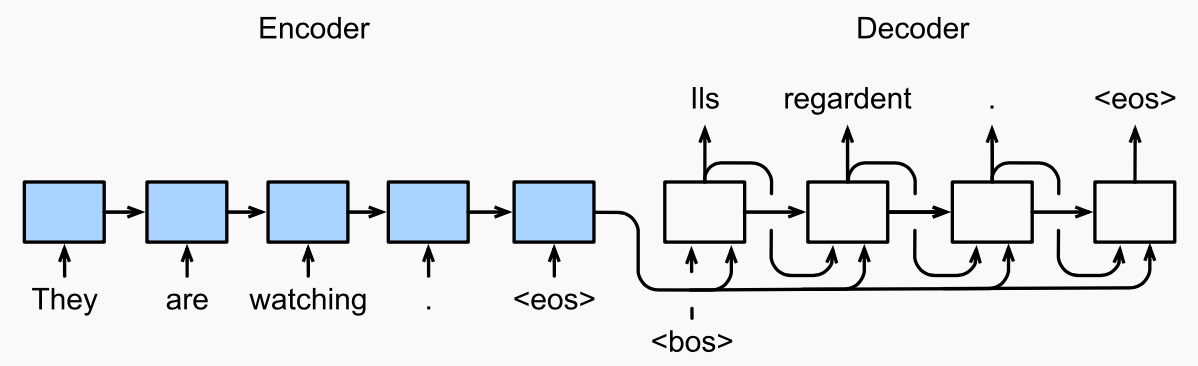
\includegraphics[height=2.5cm]{figures/rnn-enc-dec-gen}
        \caption{10.7.1 from \href{https://d2l.ai/chapter_recurrent-modern/seq2seq.html}{d2l.ai}}
    \end{figure}
        }
            \only<+->{
        Option 2: the groundtruth prefix (\textbf{teacher forcing})
    \begin{figure}
        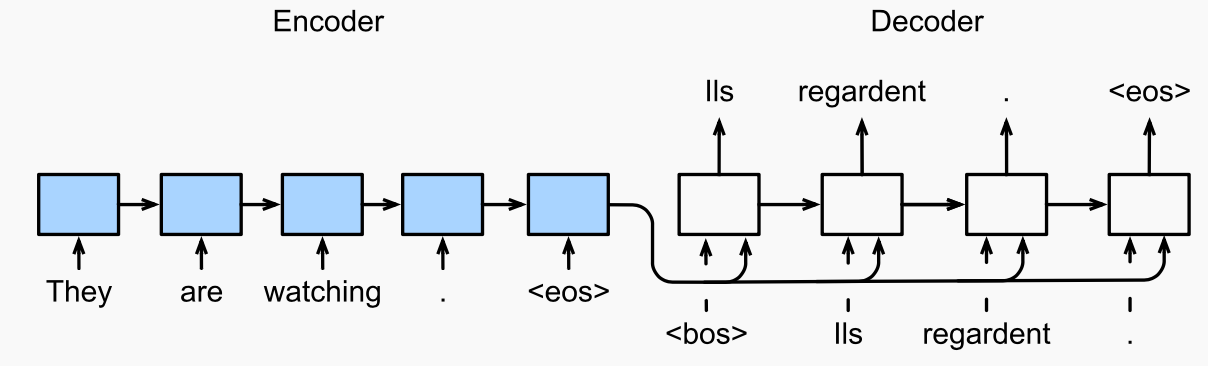
\includegraphics[height=2.5cm]{figures/rnn-enc-dec}
        \caption{10.7.3 from \href{https://d2l.ai/chapter_recurrent-modern/seq2seq.html}{d2l.ai}}
    \end{figure}
        }
\end{frame}

\begin{frame}
    {Decoder attention masking}

    Recall that the output of self-attention depends on all tokens $y_1,\ldots y_m$.

    But the decoder is supposed to model $p(y_t\mid y_{<t}, x)$.

    It should not look at the ``future'' ($y_{t+1},\ldots,y_m$)!

    \pause
    How do we fix the decoder self-attention?\\
    \begin{itemize}
        \item Mathematically, changing the input values and keys suffices.
        \item Practically, set $a(s_i, s_j)$ to $-\inf$ for all $j>i$ and for $i=1,\ldots,m$.
            \begin{itemize}
                \item The attention matrix is a lower-triangular matrix.
            \end{itemize}
    \end{itemize}
\end{frame}


\begin{frame}
    {Inference}
    How do we generate sequences given a trained model?
    \begin{figure}
        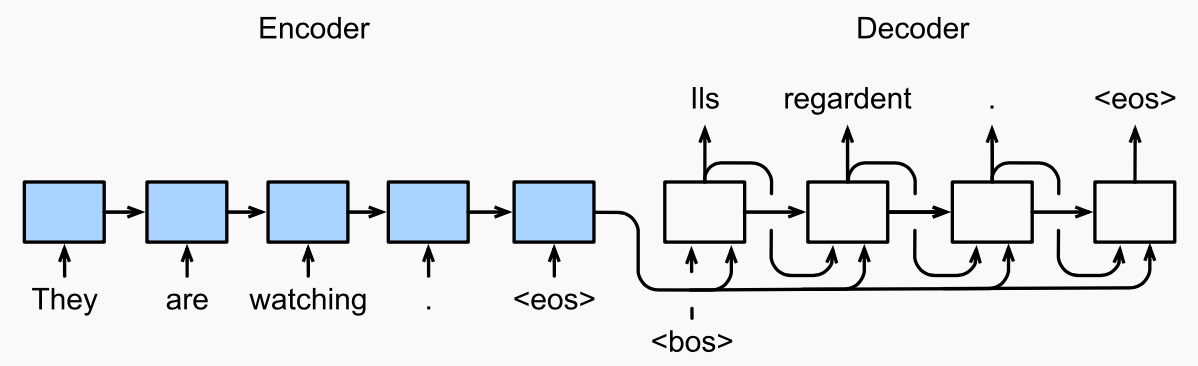
\includegraphics[height=2.5cm]{figures/rnn-enc-dec-gen}
        \caption{10.7.1 from \href{https://d2l.ai/chapter_recurrent-modern/seq2seq.html}{d2l.ai}}
    \end{figure}

    The encoder-decoder model defines a probability distribution $p(y\mid x;\theta)$ over sequences.

    Which one should we output?
\end{frame}

\begin{frame}
    {Inference}

    \textbf{Argmax decoding}: 
    $$
    \hat{y} = \argmax_{y\in\red{\sV_{\text{out}}^n}} p(y\mid x; \theta)
    $$
    \vspace{-1em}
    \begin{itemize}
        \item Return the \red{most likely sequence}
        \item But exact search is intractable 
    \end{itemize}

    \pause
    Approximate search:\\
    \begin{itemize}
        \item \textbf{Greedy decoding}: return the \green{most likely symbol} at each step
            $$
            y_t = \argmax_{y\in\green{\sV_{\text{out}}}} p(y\mid x, y_{<t}; \theta)
            $$
    \end{itemize}
\end{frame}

\begin{frame}
    {Approximate decoding: beam search}
    \textbf{Beam search}: maintain $k$ (beam size) highest-scored \blue{partial} solutions at every step 
    
    Example: $|\sV|=5, k=2$
    \vspace{-1em}
    \begin{figure}
        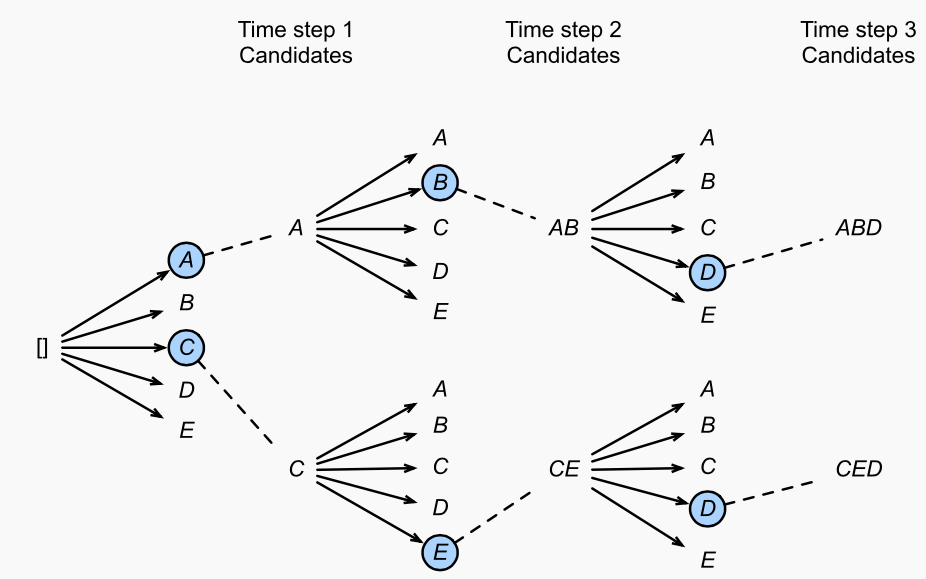
\includegraphics[height=4cm]{figures/beam-search}
    \end{figure}
    \vspace{-1em}

    \begin{itemize}
        \item At each step, rank symbols by log probability of the partial sequence
        \item Keep the top-$k$ symbol out of all possible continuations
        \item Save \textbf{backpointer} to the previous state
    \end{itemize}
\end{frame}

\begin{frame}
    {Is argmax the right decoding objective?}
    \blue{High likelihood} can be correlated with \red{low quality} outputs!
    \vspace{-1em}
    \begin{figure}
        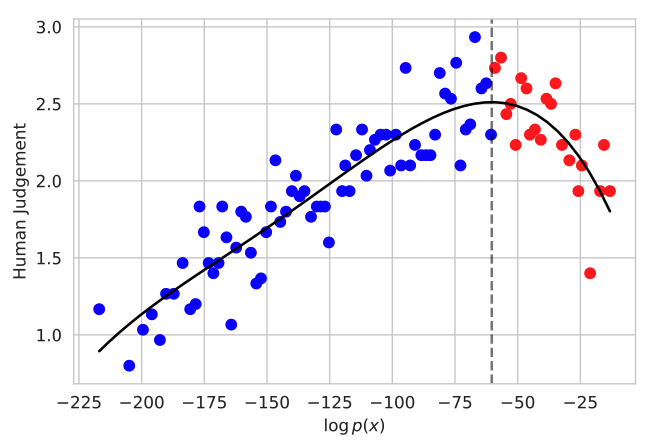
\includegraphics[height=3cm]{figures/likelihood-trap}
        \caption{From the \href{https://arxiv.org/abs/2004.10450}{likelihood trap} paper by Zhang et al., 2020}
    \end{figure}
    \vspace{-2em}

    In practice, argmax decoding has been observed to lead to\\
    \begin{itemize}
        \item Repetitive generations, e.g.\\
            {\footnotesize
                ``..., was conducted by researchers from the Universidad Nacional Autonoma de Mexico (UNAM) and \textcolor{red}{the Universidad Nacional Autonoma de Mexico (UNAM/Universidad Nacional Autonoma de Mexico/Universidad Nacional Autonoma de Mexico/Universidad Nacional Autonoma...}''}
        \item Degraded generations with large beam size in MT
    \end{itemize}
\end{frame}

\begin{frame}
    {Sampling-based decoding}
    If we have learned a perfect $p(y\mid x)$, shouldn't we just sample from it?

    \textbf{Sampling} the next word sequentially:\\
    \begin{itemize}
        \item While output is not \texttt{EOS}
            \begin{itemize}
                \item Sample next word from $p(\cdot\mid \text{prefix}, \text{input};\theta)$
                \item Append the word to prefix
            \end{itemize}
    \end{itemize}

    \pause
    Standard sampling often produces non-sensical sentences:\\
    \begin{itemize}
        \item[] {\footnotesize They were cattle called Bolivian Cavalleros; they live in a remote desert uninterrupted by town, and they speak huge, beautiful, paradisiacal Bolivian linguistic thing.}
    \end{itemize}

    Typically we modify the learned distrubtion $p_\theta$ before sampling the next word
\end{frame}

\begin{frame}
    {Tempered sampling}

    \textbf{Intuition}: concentrate probability mass on highly likely sequences 

    Scale scores (from the linear layer) before the softmax layer:\\
    \begin{align*}
        p(y_t=w \mid y_{<t},x) &\propto \exp\p{\mathrm{score}(w)}\\
        q(y_t=w \mid y_{<t}, x) &\propto \exp\p{\mathrm{score}(w)/{\color{blue}T}} 
        \quad \text{where } T\in(0, +\infty)
    \end{align*}
    \pause
    \vspace{-2em}
    \begin{itemize}
        \item What happends when $T\to 0$ and $T\to +\infty$?
        \item Does it change the rank of $y$ according to likelihood?
        \item Typically we chooose $T\in (0, 1)$, which makes the distribution more peaky.
    \end{itemize}
\end{frame}

\begin{frame}
    {Truncated sampling}

    Another way to focus on high likelihood sequences: \blue{truncate the tail} of the distribution

    \textbf{Top-k sampling}:\\
    \begin{itemize}
        \item Rank all tokens $w\in\sV$ by $p(y_t=w\mid y_{<t},x)$
        \item Only keep the top $k$ of those and renormalize the distribution
    \end{itemize}

    \pause
    Which $k$ to choose?
    \vspace{-1em}
    \begin{figure}
        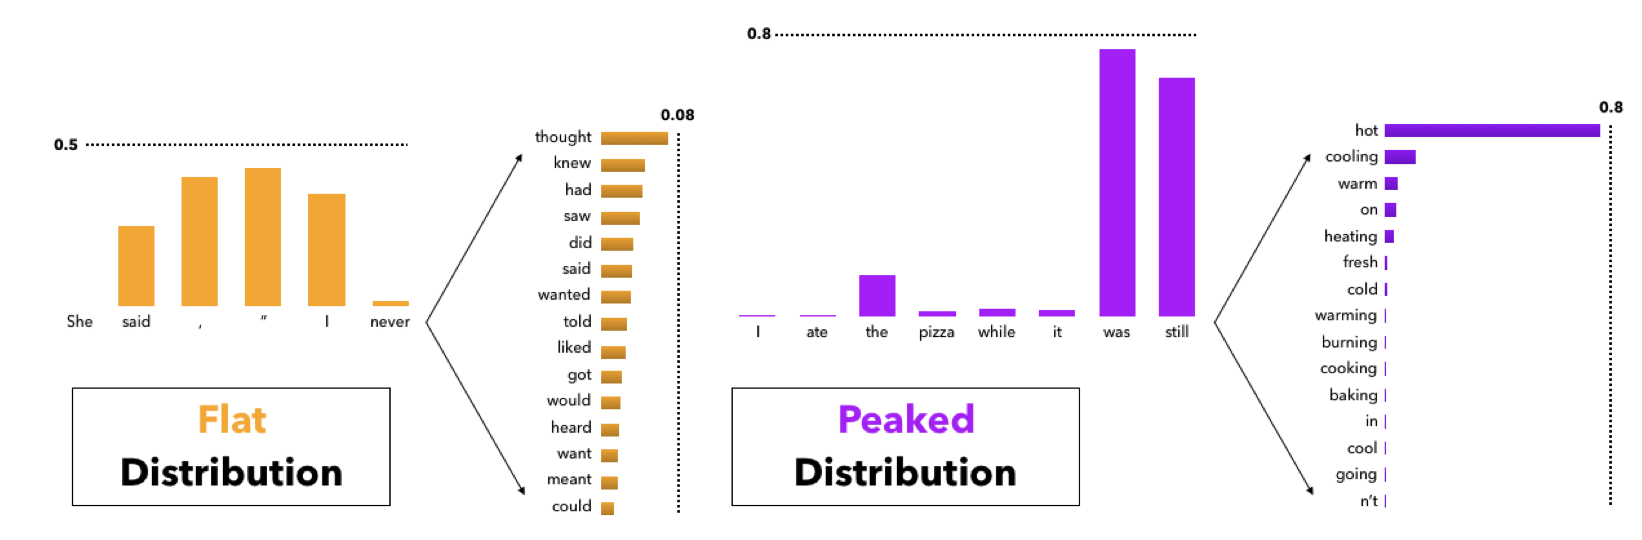
\includegraphics[height=3cm]{figures/dynamic-k}
        \caption{From the \href{https://arxiv.org/pdf/1904.09751.pdf}{nucleus sampling} paper by Holtzman et al., 2020}
    \end{figure}
\end{frame}

\begin{frame}
    {Truncated sampling}
    
    \textbf{Top-p sampling}:
    \begin{itemize}
        \item Rank all tokens $w\in\sV$ by $p(y_t=w\mid y_{<t},x)$
        \item Keep only tokens in the top $p$ probability mass
            and renormalize the distribution
        \item The corresponding $k$ is dynamic:
            \begin{itemize}
            \item Start with $k=1$, increment until the cumulative probability mass is larger than $p$
            \end{itemize}
    \end{itemize}
\end{frame}

\begin{frame}
    {Decoding in practice}
    \begin{itemize}
        \item Can combine different tricks (e.g., temperature + beam search, temperature + top-$k$)
        \item Use beam search with small beam size for tasks where there exists a correct answer, e.g. machine translation, summarization
        \item Use top-$k$ or top-$p$ for open-ended generation, e.g. story generation, chit-chat dialogue, continuation from a prompt
        \item As models getting better/larger, sampling-based methods tend to work better
    \end{itemize}
\end{frame}

\end{document}
